% !Mode:: "TeX:UTF-8" 

\section{测试样张}

\subsection{测试1}

\subsubsection{参考文献引用测试}
\indent 本学位论文作者完全了解江南大学有关保留、使用学位论文的规定:江南大学有权保留并向国家有关部门或机构送交论文的复印件和电子版,允许论文被查阅和借阅,可以将学位论文的全部或部分内容编入有关数据库进行检索,可以采用影印、缩印或扫描等复制手段保存、汇编学位论文,并且本人电子文档的内容和纸质论文的内容相一致。

\subsubsection{表格测试}
\begin{table}[htbp]
	\centering
	\caption{算法在$ wellseparatednoise $上的总相似度均值与标准差}
	\setlength{\tabcolsep}{3mm}{
		\begin{tabular}{c lllllllllllllllllllll}
			\hline
			{K} & {改进KM} &{改进AP} &{混合算法} &{ALC}&{GrC}\\
			\hline
			{1} & \textbf{-10938.0 (0.0)} & -11097.5 (29.8) & -10938.2 (0.0) & -18904.9 (0.0) & -18905.0 (0.0) \\
			{2} & \textbf{-5552.4 (0.0)} & -5609.1 (12.8) & -5552.4 (0.0) & -7575.0 (0.0) & -18428.0 (0.0) \\
			{3} & \textbf{-3345.5 (0.0)} & -3365.7 (23.4) & -3345.5 (0.0) & -3723.5 (0.0) & -15316.2 (227.1) \\
			{4} & -2882.5 (0.0) & -2925.7 (12.3) & -2885.8 (4.0)  & -4450.0 (0.0) & -15319.7 (223.7) \\
			{5} & -2973.4 (0.0) & -3014.4 (2.7) & -2973.6 (0.4)  & -5116.5 (0.0) & -15763.5 (110.7) \\
			{6} & \textbf{-3534.7 (0.0)} & -3811.5 (6.7) & -3668.9 (38.9)  & -5638.2 (0.0) & -15413.0 (0.0) \\
			{7} & \textbf{-4315.1 (2.4)} & -4665.1 (3.2) & -4522.8 (0.0)& -6623.3 (0.0) & -16075.0 (27.8) \\
			{8} & \textbf{-5183.1 (3.9)} & -5415.0 (0.0) & -5362.3 (71.4) & -7530.5 (0.0) & -12356.3 (1693.0) \\
			{9} & \textbf{-6088.2 (1.8)} & -6293.3 (4.8) & -6176.0 (11.2)& -8232.0 (0.0) & -12554.0 (0.0) \\
			{10} & \textbf{-6999.3 (6.5)} & -7112.1 (6.4) & -7032.0 (7.1)  & -9119.2 (0.0) & -13120.4 (0.2) \\
			\hline
	\end{tabular}}
\end{table}

\subsubsection{图片测试}
\begin{figure}[H]
	\centering
	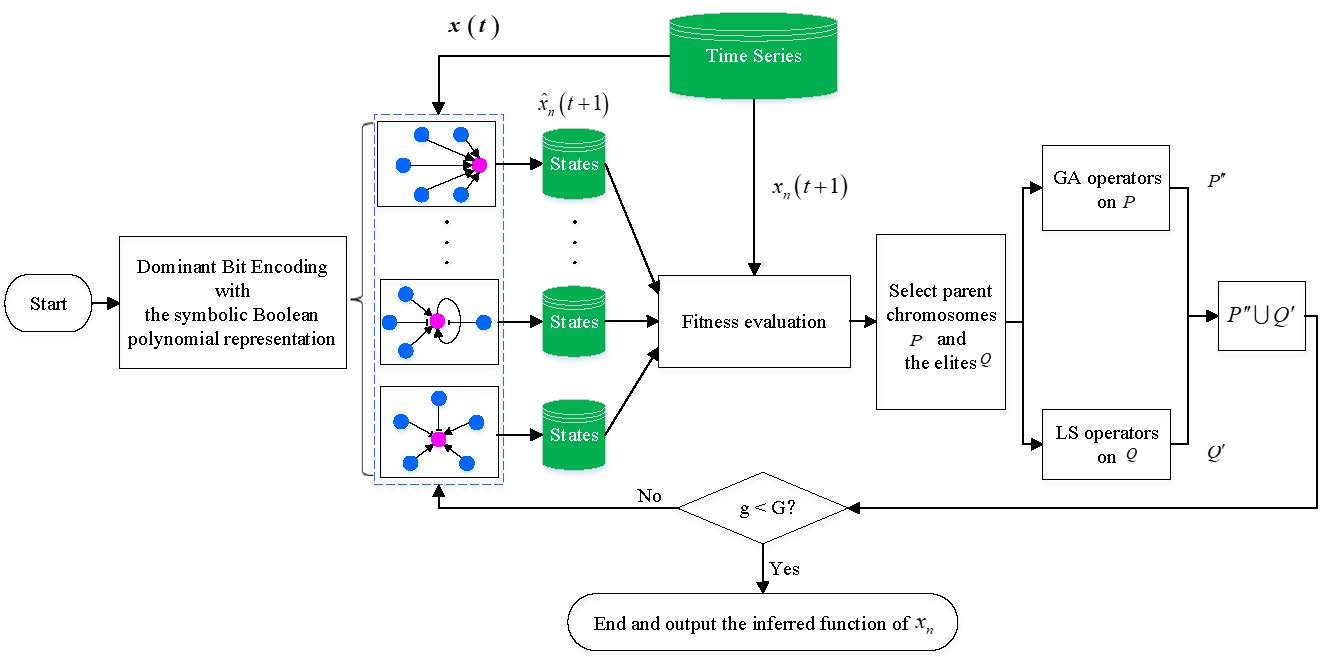
\includegraphics[width=0.9\linewidth]{image/GAPORE}
	\caption{测试}
	\label{fig:gapore}
\end{figure}




\subsection{测试2}

\subsubsection{定理测试}
\begin{theorem}[勾股定理]
	若 $a,b$ 为直角三角形的两条直角边,$c$ 为斜边,那么 $a^2 + b^2 + c^2.$
\end{theorem}

\begin{definition}[勾股定理]
	若 $a,b$ 为直角三角形的两条直角边,$c$ 为斜边,那么 $a^2 + b^2 + c^2.$
\end{definition}


\subsubsection{公式测试}
\begin{small}
	\begin{equation}
		\left\{
		\begin{array}{*{20}{c}}\label{E2}
			{{\hat{x}_1}\left( {t + 1} \right) = {\hat{f}_{1}}\left( {{\hat{x}_{1_{1}}}\left( t \right),{\hat{x}_{1_{2}}}\left( t \right), \cdots ,{\hat{x}_{{1_{K_1}}}}\left( t \right)} \right)}\\
			\vdots \\
			{{\hat{x}_n}\left( {t + 1} \right) = {\hat{f}_{n}}\left( {{\hat{x}_{n_{1}}}\left( t \right),{\hat{x}_{n_{2}}}\left( t \right), \cdots ,{\hat{x}_{{n_{K_n}}}}\left( t \right)} \right)}\\
			\vdots \\
			{{\hat{x}_N}\left( {t + 1} \right)   = {\hat{f}_{N}}\left( {{\hat{x}_{N_{1}}}\left( t \right),{\hat{x}_{N_{2}}}\left( t \right), \cdots ,{\hat{x}_{{N_{K_N}}}}\left( t \right)} \right)}
		\end{array}
		\right.
	\end{equation}
	
	\begin{eqnarray}
		&&x_{n}(t+1)= f\left ( x_{n_1}(t), x_{n_2}(t),\cdots, x_{n_K}(t) \right )\nonumber\\
		&&= a_{0}+a_{1}x_{n_1}(t)+a_{2}x_{n_2}(t)+a_{3}x_{n_1}(t)x_{n_2}(t)+a_{4}x_{n_3}(t)\nonumber\\
		&&+a_{5}x_{n_1}(t)x_{n_3}(t)+a_{6}x_{n_2}(t)x_{n_3}(t)+a_{7}x_{n_1}(t)x_{n_2}(t)x_{n_3}(t)\nonumber\\
		&&+\cdots+a_{2^K-1}x_{n_1}(t)x_{n_2}(t)\cdots x_{n_{K}}(t)\nonumber\\
		&&=\sum_{i=0}^{2^K-1} a_{i}x_{n_{1}}^{b_{1}}(t) x_{n_2}^{b_2}(t) \cdots x_{n_{K}}^{b_{K}}(t)   \label{En}
	\end{eqnarray}
	
	\begin{equation}
		\left\{
		\begin{aligned}
			& x_{16} (t+1) = x_{16}(t) \\
			& x_{17} (t+1) = [x_{29}(t) \wedge x_{16}(t)  \wedge  \neg x_{30}(t)] \\
			&\vee [x_{17}(t) \wedge(x_{29}(t) \vee x_{16}(t))] \wedge \neg x_{30}(t) \\
			& x_{18} (t+1) = x_{17}(t) \\
			& x_{19} (t+1)=  \neg x_{16}(t)  \wedge [x_{3}(t)   \vee  x_{33}(t)]  \\
			& x_{20} (t+1)= x_{19}(t)  \\
			& x_{21} (t+1)=  \neg x_{30}(t)  \wedge x_{20}(t)  \\
			& x_{22} (t+1)= x_{21}(t)  \\
			& x_{23} (t+1)=  \neg x_{30}(t) \wedge  \neg x_{20}(t)  \wedge x_{29}(t)  \\
			& x_{24} (t+1)= x_{23}(t)  \vee  [x_{24}(t)  \wedge  \neg x_{7}(t)  \wedge  \neg x_{37}(t)] \\
			& x_{25} (t+1)= [x_7(t) \vee  x_{37}(t)]  \wedge x_{24}(t)  \\
			& x_{26} (t+1)=  \neg x_{24}(t)   \vee  [x_7(t)   \vee  x_{37}(t)]  \\
			& x_{27} (t+1)=  \neg x_{20}(t)  \\
			& x_{28} (t+1)=  x_{27}(t)  \\
			& x_{29} (t+1)=  x_{28}(t)  \wedge [x_{26}(t)  \vee  x_{6}(t)  \vee x_{36}(t)] \\
			& x_{30} (t+1)=  \neg x_{26}(t)  \wedge  \neg x_{6}(t)  \wedge  \neg x_{36}(t)  \wedge x_{28}(t) \\
		\end{aligned}
		\label{SegmentBF}
		\right.
	\end{equation}
\end{small}





\clearpage